\chapter{Background}
This chapter will begin by summarizing the most common types web application security vulnerabilities. Next, it will define and describe \acrfull{waf}s, which are used to defend against these vulnerabilities. This section will also include a \acrfull{mlr} that was conducted to determine how \acrshort{waf}s are mostly commonly bypassed and then map those evasion techniques to common vulnerability types. Then, various \acrfull{ai} and \acrfull{ml} methods for detecting and/or preventing attacks against a \acrshort{waf} will be described. Afterwards, some background will be given on code generation and model-driven development. Finally, the last section will summarize the state-of-the-art for model-driven security.

\section{Common Web Security Vulnerabilities}
The \acrfull{owasp} maintains a list of "The Ten Most Critical Web Application Security Risks" called OWASP Top 10 \cite{owasp2017top}. The OWASP Top 10 2017 release relied on what is possibly the most amount of data ever collected for developing an application security standard \cite{owasp2017top}. These vulnerabilities will be referred to by ID (e.g., A1 for Injection) and/or name throughout the rest of this paper.

\begin{figure}[htbp]  % order of priority: h here, t top, b bottom, p page
  \centering
  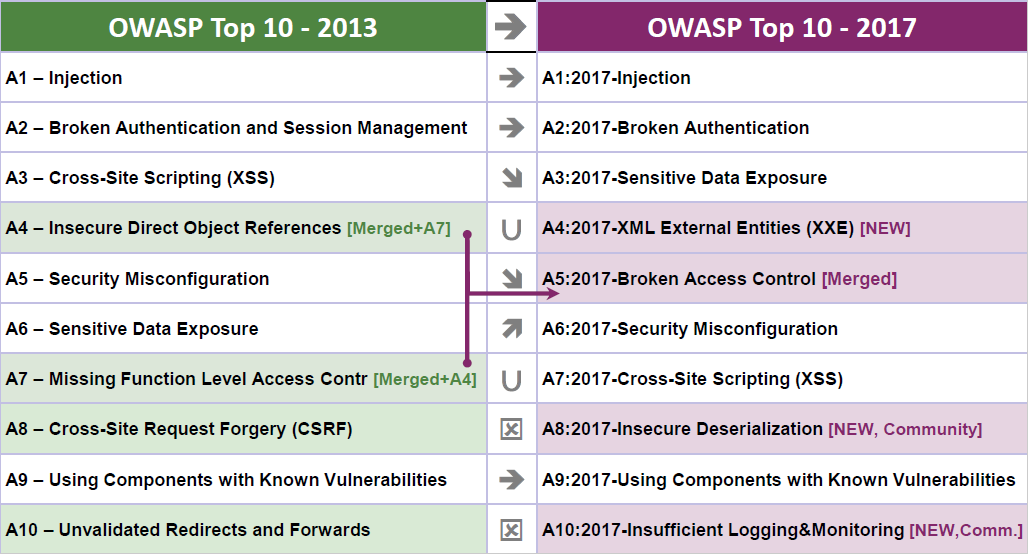
\includegraphics[width=.55\textwidth]{figures/owasp_2013_2017.png}
  \caption[OWASP Top 10]{A comparison of OWASP Top 10 - 2017 with the 2013 edition \cite{owasp2017top}.}
  \label{fig:owasp_2013_2017}
\end{figure}

\section{Web Application Firewalls}
A \acrfull{waf} is an application-level firewall that can be deployed to protect one or more web applications \cite{owasp_waf}. It generally runs in front of a web server through a reverse proxy \cite{owasp_waf}, and it monitors, filters, and blocks packets of data as they travel to/from a web application \cite{techtarget_waf}. \acrshort{waf}s can be categorized in terms of deployment (hardware, software, or cloud)\cite{pentasecurity_types}, security model (positive/whitelist, negative/blacklist, or hybrid)\cite{techtarget_waf}, threat detection system (signature or rule-based)\cite{pentasecurity_tds}, and license type (commercial or open-source). Gartner's Magic Quadrant for Web Application Firewalls provides a list of the most important and relevant commercial solutions in the market \cite{gartner2020}. ModSecurity along with the \acrshort{owasp} \acrfull{crs} is a major open-source solution \cite{owasp_crs}.

\begin{figure}[htbp]  % order of priority: h here, t top, b bottom, p page
  \centering
  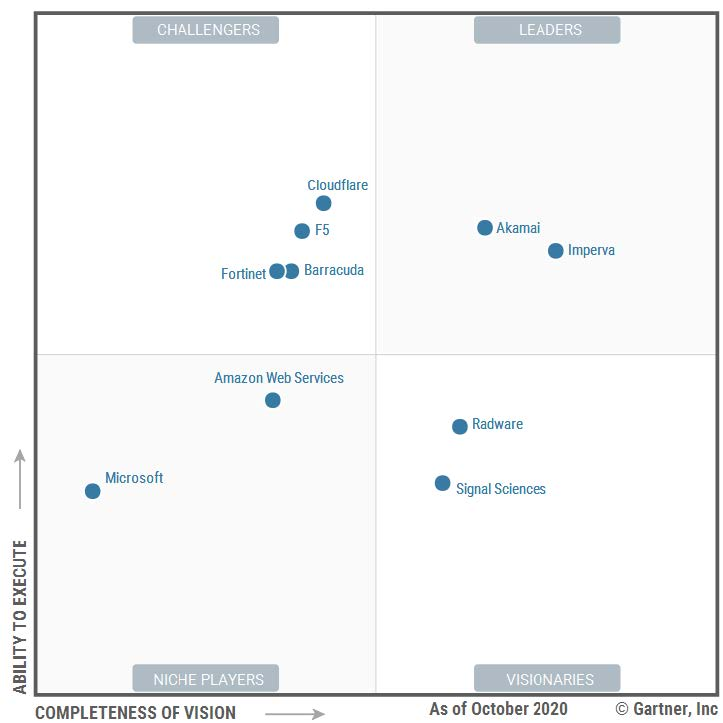
\includegraphics[width=.6\textwidth]{figures/gartner_wafs_2020.jpg}
  \caption[Gartner WAF 2020]{Magic Quadrant for Web Application Firewalls \cite{gartner2020}.}
  \label{fig:gartner_wafs_2020}
\end{figure}

\subsection{\acrshort{waf} Strengths and Weaknesses}
In order to determine which types of attacks the above \acrshort{waf}s were most and least effective against, a \acrshort{mlr} was conducted following a set of guidelines designed for software engineering \cite{garousi2019guidelines}. 

\subsubsection{Planning the review}
First, it needed to be determined whether or not a \acrshort{mlr} was actually needed. After a few manual searches using Scopus, Google Scholar, and Google, the following questions \cite{garousi2019guidelines} were answered:

\begin{figure}[htbp]  % order of priority: h here, t top, b bottom, p page
  \centering
  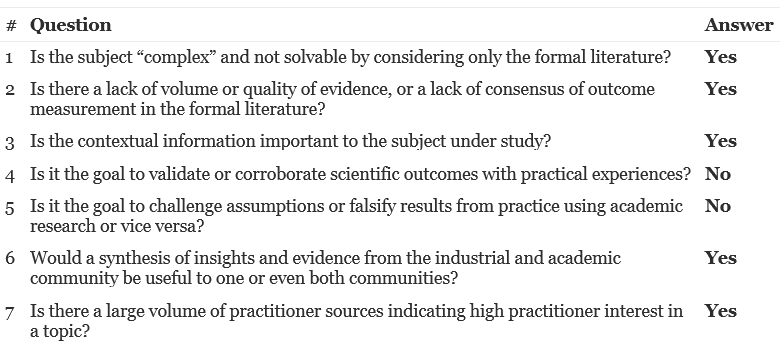
\includegraphics[width=.8\textwidth]{figures/planning_review_1.png}
  \caption[MLR Question]{Should I conduct an \acrshort{mlr}?}
  \label{fig:planning_review_1}
\end{figure}

Since most answers were yes, an \acrshort{mlr} is appropriate. Next, a research/review question with sub-questions was formulated:

\begin{enumerate}
    \item How many studies have evaluated \acrshort{waf}s in terms of the types of attacks they are able to protect against?
    \begin{enumerate} 
        \item Which \acrshort{waf}s have been evaluated?
        \item Which types of attacks are most effective, and how do they map to OWASP’s Top 10 Web Application Security Risks?
    \end{enumerate}
\end{enumerate}

\subsubsection{Conducting the review}
\textbf{The following search engine(s) were used for academic/formal literature}:
\begin{itemize}
    \item Scopus
    \item Google Scholar
\end{itemize}

\textbf{The following search engine(s) were used for gray literature}:
\begin{itemize}
    \item Google
\end{itemize} 

\textbf{Stopping criteria:}
\begin{itemize}
    \item First 50 search hits
    \item Continue only if last page reveals anything new or interesting
\end{itemize}

\textbf{Inclusion criteria:}
\begin{itemize}
    \item Discusses the effectiveness of an attack/attacks against an available WAF/WAFs 
    \item Comprehensible English
    \item 2014 or newer
\end{itemize}

\textbf{Query:}

\texttt{"web application firewall" AND  (fail  OR  survey  OR  comparison  OR  "false negative" OR  "evade"  OR  "evasion"  OR  "bypass" OR detect)}
\\\\
Taking into account the stopping and inclusion criteria, there were only 13 results. Thus, it was decided to repeat the following query for every WAF listed in \cite{gartner2020} (starting with Amazon) and ModSecurity:

\texttt{"amazon" "application firewall" "bypass"}
\\\\
This yielded an additional 22 results once the stopping and inclusion criteria were applied.

\subsubsection{Results}
Table \ref{Tab:successful_attacks} shows which types of attacks were able to successfully bypass a given \acrshort{waf}. The attacks are categorized by OWASP Top 10 - 2017 categories. An x means that a type of attack indicated by the column was successful against the \acrshort{waf} indicated by a row, i.e., the \acrshort{waf} was bypassed. \acrfull{lfirfi} is also a category.

\begin{table}[!htbp]
\begin{tabular}{|l|c|c|c|c|c|c|c|c|c|c|c|}
\hline
& \multicolumn{10}{c|}{\textbf{OWASP Top 10 - 2017}} &
\\ \hline
\textbf{WAF}      & \multicolumn{1}{l|}{\textbf{A1}} & \multicolumn{1}{l|}{\textbf{A2}} & \multicolumn{1}{l|}{\textbf{A3}} & \multicolumn{1}{l|}{\textbf{A4}} & \multicolumn{1}{l|}{\textbf{A5}} & \multicolumn{1}{l|}{\textbf{A6}} & \multicolumn{1}{l|}{\textbf{A7}} & \multicolumn{1}{l|}{\textbf{A8}} & \multicolumn{1}{l|}{\textbf{A9}} & \multicolumn{1}{l|}{\textbf{A10}} & \multicolumn{1}{l|}{\textbf{LFI/RFI}} \\ \hline
Akamai & x &  &  & & & & x & & & &
\\ \hline
Amazon & & & & & & & & & & &
\\ \hline
Barracuda & & x & & & & & x & & & &
\\ \hline
Cloudflare & x & & & & & x & x & & & &
\\ \hline
Comodo & x & & & & & x & & & & & x
\\ \hline
Fortinet & & & & & & & & & & &
\\ \hline
F5 Big IP & x & & & & x & & x & x & & &
\\ \hline
Guardian & x & & & & x & x & x & & & & x
\\ \hline
Imperva Incapsula & & & & & & & x & & & &
\\ \hline
Microsoft Azure & & & & & & & & & & &
\\ \hline
ModSecurity & x & x & & & x & x & x & & & x & x
\\ \hline
PHPIDS & x & & & & & x & & & & & x
\\ \hline
QuickDefense & x & & & & & x & x & & & & x
\\ \hline
Radware & & & & & & & & & & &
\\ \hline
Signal Sciences & & & & & & & & & & &
\\ \hline
Sucuri & x & & & & & x & x & & & &
\\ \hline
WebKnight & x & & & & x & x & x & & & &
\\ \hline

\end{tabular}
  \caption{Successful attacks against WAFs categorized by OWASP Top 10 - 2017.}
  \label{Tab:successful_attacks}
\end{table}
Tables \ref{Tab:papers_owasp} and \ref{Tab:papers_waf} show the number of formal and gray papers that pertained to each \acrshort{waf} and each OWASP Top 10 - 2017 category.
\begin{table}[!htbp]
\begin{tabular}{|l|r|r|r|}
\hline
\textbf{OWASP Top 10 - 2017}
& \textbf{Formal Papers}
& \textbf{Gray Papers}
& \textbf{Total}
\\ \hline
A1 & 11 & 12 & 23
\\ \hline
A2 & 2 & 1 & 3
\\ \hline
A3 & 0 & 0 & 0
\\ \hline
A4 & 0 & 0 & 0
\\ \hline
A5 & 5 & 1 & 6
\\ \hline
A6 & 1 & 5 & 6
\\ \hline
A7 & 3 & 7 & 10
\\ \hline
A8 & 0 & 1 & 1
\\ \hline
A9 & 0 & 0 & 0
\\ \hline
A10 & 1 & 0 & 1
\\ \hline
LFI/RFI & 3 & 1 & 4
\\ \hline

\end{tabular}
  \caption{Number of papers that pertaining to each OWASP Top 10 - 2017 category.}
  \label{Tab:papers_owasp}
\end{table}

\begin{table}[!htbp]
\begin{tabular}{|l|r|r|r|}
\hline
\textbf{WAF}
& \textbf{Formal Papers}
& \textbf{Gray Papers}
& \textbf{Total}
\\ \hline
Akamai & 0 & 3 & 3
\\ \hline
Amazon & 0 & 0 & 0
\\ \hline
Barracuda & 0 & 2 & 2
\\ \hline
Cloudflare & 0 & 9 & 9
\\ \hline
Comodo & 0 & 1 & 1
\\ \hline
Fortinet & 0 & 0 & 0
\\ \hline
F5 Big IP & 0 & 5 & 5
\\ \hline
Guardian & 1 & 0 & 1
\\ \hline
Imperva Incapsula & 0 & 2 & 2
\\ \hline
Microsoft Azure & 0 & 0 & 0
\\ \hline
ModSecurity & 12 & 9 & 21
\\ \hline
PHPIDS & 1 & 2 & 3
\\ \hline
QuickDefense & 0 & 2 & 2
\\ \hline
Radware & 0 & 0 & 0
\\ \hline
Signal Sciences & 0 & 0 & 0
\\ \hline
Sucuri & 0 & 4 & 4
\\ \hline
WebKnight & 1 & 2 & 3
\\ \hline

\end{tabular}
  \caption{Number of papers that pertaining to each WAF.}
  \label{Tab:papers_waf}
\end{table}


\subsection{Evasion strategies}
There are many strategies for evading \acrshort{waf} protections. For XSS, many involve encoding or obfuscation of the malicious script. The obfuscation can be a syntax error, an obscure encoding, or an esoteric subset of Javascript like JSFuck. Others require the usage of obscure or obsolete HTML attributes and events \cite{owasp_bypass_techniques}.

Mimicry JavaScript attacks, a variation of XSS attacks. Uses slight transformations (i.e., changing the leaf values of abstract syntax tree) of an application’s benign scripts as attack vectors for malicious purposes. This bypasses WAFs that use script-whitelisting mechanisms. Script-whitelisting mechanisms creates unique identifiers for every valid script during a training phase, which takes place before an app goes live. These identifiers combine elements that are extracted from either the script, i.e., part of the AST, or its execution env, such as the URL that triggered execution. The identifiers are stored in a whitelist. During productions, only scripts that generate identifiers in the whitelist will be identified and approved for execution. \cite{chaliasos2019mime}

\subsection{Improving detection of attacks}
Previous studies have proposed anomaly detectors based on characteristics of HTTP requests such as character distribution, parameter length, and parameter value. TokDoc is a \acrshort{waf} that analyzes HTTP requests and replaces suspicious parts with benign pieces learned from the past \cite{krueger2010tokdoc}. One recent study uses session patterns \cite{tanriverdi2019implementation}. Others use such approaches as the Random Forest Method \cite{thang2020improving} and feature analysis and SVM optimization \cite{liu2020web}. 

It has been shown that it often takes more time to manually configure a \acrshort{waf} than it takes for a tester or hacker to bypass it \cite{virtualpatching}, \cite{virtualpatching_survey}. Thus, researchers have started to develop ways to automatically configure and repair them. \cite{appelt2017automatically} proposes an approach to automatically repair vulnerable \acrshort{waf}s by augmenting existing rulesets based on an analysis of test results, using machine learning and metaheuristics. The focus was SQL injection attacks since they sit atop OWASP Top 10.

%\section{Automatic Fixing of Vulnerabilities}
%As opposed to relying on a \acrshort{waf} which can be bypassed as mentioned in previous sections, security vulnerabilities within %the code can be fixed. \cite{marchand2020automatic} was a survey of 20 papers that proposed some solution for automatically %detecting and fixing vulnerabilities classified by OWASP Top 10. The target languages were either PHP or Java, and the three most %popular vulnerabilities to address were A1 (injection), A7 (XSS), and A3 (sensitive data exposure). Of particular interest is 
\section{Code Generation}

\section{Model-Driven Security}